%! TeX program = lualatex
\documentclass[a4paper,11pt]{article} 
% packages
\usepackage{censor}
\usepackage{multicol}
\usepackage{algorithm}
\usepackage{algpseudocode}
\StopCensoring
\usepackage{fontspec}
\setmainfont{EB Garamond}
% for tironian et fallback
% % \directlua{luaotfload.add_fallback
% % ("emojifallback",
% %      {"Noto Serif:mode=harf"}
% % )}
% % \setmainfont{EB Garamond}[RawFeature={fallback=emojifallback}]

\setmonofont[Scale=MatchLowercase]{Deja Vu Sans Mono}
\usepackage[a4paper,left=2cm,right=2cm,top=\dimexpr15mm+1.5\baselineskip,bottom=2cm]{geometry}
\setlength{\parindent}{0pt}

\usepackage{tcolorbox}
\usepackage{amsmath}
\usepackage{fancyhdr}       % Headers and footers 
\fancyhead[R]{\normalfont \leftmark}
\fancyhead[L]{}
\pagestyle{fancy}

\usepackage{microtype}      % Slightly tweak font spacing for aesthetics
\usepackage[english]{babel} % Language hyphenation and typographical rules
\usepackage{xcolor}
\setlength{\fboxsep}{0pt}
\definecolor{linkblue}{RGB}{0, 64, 128}
\usepackage[final, colorlinks = false, urlcolor = linkblue]{hyperref} 
% \newcommand{\secref}[1]{\textbf{§~\nameref{#1}}}
\newcommand{\secref}[1]{\textbf{§\ref{#1}~\nameref{#1}}}

\usepackage{changepage}     % adjust margins on the fly

\usepackage{minted}
\usemintedstyle{algol_nu}

\usepackage{pgfplots}
\pgfplotsset{width=\textwidth,compat=1.9}

\usepackage{caption}
\newenvironment{code}{\captionsetup{type=listing}}{}
\captionsetup[listing]{skip=0pt}
\setlength{\abovecaptionskip}{5pt}
\setlength{\belowcaptionskip}{5pt}

\usepackage[yyyymmdd]{datetime}
\renewcommand{\dateseparator}{--}

\usepackage[bottom]{footmisc}
\renewcommand{\footnoterule}{%
    \hrule
    \vspace{5pt}
}

% Remove superscript from footnote numbering
% \renewcommand{\thefootnote}{\arabic{footnote}} % Use Arabic numbers
% \renewcommand{\footnotelabel}{\thefootnote. } % Footnote label formatting

\usepackage{enumitem}

\usepackage{titlesec}

\author{Andrew Hayes}

\begin{document}
\begin{titlepage}
    \begin{center}
        \hrule
        \vspace*{0.6cm}
        \censor{\huge \textbf{CT4101}}
        \vspace*{0.6cm}
        \hrule
        \LARGE
        \vspace{0.5cm}
            Machine Learning
        \vspace{0.5cm}
        \hrule

        \vfill
        \vfill

        \hrule
        \begin{minipage}{0.495\textwidth} 
            \vspace{0.4em}
            \raggedright
            \normalsize 
            Name: Andrew Hayes \\
            E-mail: \href{mailto://a.hayes18@universityofgalway.ie}{\texttt{a.hayes18@universityofgalway.ie}}  \hfill\\   
            Student ID: 21321503 \hfill
        \end{minipage}
        \begin{minipage}{0.495\textwidth} 
            \raggedleft
            \vspace*{0.8cm}
            \Large
            \today
            \vspace*{0.6cm}
        \end{minipage}
        \medskip\hrule 
    \end{center}
\end{titlepage}

\pagenumbering{roman}
\newpage
\tableofcontents
\newpage
\setcounter{page}{1}
\pagenumbering{arabic}

\section{Introduction}
\subsection{Lecturer Contact Details}
\begin{itemize}
    \item   Dr. Frank Glavin.
    \item   \href{mailto://frank.glavin@universityofgalway.ie}{\texttt{frank.glavin@universityofgalway.ie}}
\end{itemize}

\subsection{Grading}
\begin{itemize}
    \item   Continuous Assessment: 30\% (2 assignments, worth 15\% each).
    \item   Written Exam: 70\% (Last 2 year's exam papers most relevant).
\end{itemize}

\subsection{Module Overview}
\textbf{Machine Learning (ML)} allows computer programs to improve their performance with experience (i.e., data).
This module is targeted at learners with no prior ML experience, but with university experience of mathematics \& 
statistics and \textbf{strong} programming skills.
The focus of this module is on practical applications of commonly used ML algorithms, including deep learning 
applied to computer vision.
Students will learn to use modern ML frameworks (e.g., scikit-learn, Tensorflow / Keras) to train \& evaluate 
models for common categories of ML task including classification, clustering, \& regression.

\subsubsection{Learning Objectives}
On successful completion, a student should be able to:
\begin{enumerate}
    \item   Explain the details of commonly used Machine Learning algorithms.
    \item   Apply modern frameworks to develop models for common categories of Machine Learning task, including
            classification, clustering, \& regression.
    \item   Understand how Deep Learning can be applied to computer vision tasks.
    \item   Pre-process datasets for Machine Learning tasks using techniques such as normalisation \& feature 
            selection.
    \item   Select appropriate algorithms \& evaluation metrics for a given dataset \& task.
    \item   Choose appropriate hyperparameters for a range of Machine Learning algorithms.
    \item   Evaluate \& interpret the results produced by Machine Learning models.
    \item   Diagnose \& address commonly encountered problems with Machine Learning models.
    \item   Discuss ethical issues \& emerging trends in Machine Learning.
\end{enumerate}

\section{What is Machine Learning?}
There are many possible definitions for ``machine learning'':
\begin{itemize}
    \item   Samuel, 1959: ``Field of study that gives computers the ability to learn without being explicitly 
            programmed''.
    \item   Witten \& Frank, 1999: ``Learning is changing behaviour in a way that makes \textit{performance} better
            in the future''.
    \item   Mitchelll, 1997: ``Improvement with experience at some task''. 
            A well-defined ML problem will improve over task $T$ with regards to \textbf{performance} measure $P$,
            based on experience $E$.
    \item   Artificial Intelligence $\neq$ Machine Learning $\neq$ Deep Learning.
    \item   Artificial Intelligence $\not \supseteq$ Machine Learning $\not \supseteq$ Deep Learning.
\end{itemize}

Machine Learning techniques include:
\begin{itemize}
    \item   Supervised learning.
    \item   Unsupervised learning.
    \item   Semi-Supervised learning.
    \item   Reinforcement learning.
\end{itemize}

Major types of ML task include:
\begin{enumerate}
    \item   Classification.
    \item   Regression.
    \item   Clustering.
    \item   Co-Training.
    \item   Relationship discovery.
    \item   Reinforcement learning.
\end{enumerate}

Techniques for these tasks include:
\begin{enumerate}
    \item   \textbf{Supervised learning:}
            \begin{itemize}
                \item   \textbf{Classification:} decision trees, SVMs.
                \item   \textbf{Regression:} linear regression, neural nets, $k$-NN (good for classification too).
            \end{itemize}

    \item   \textbf{Unsupervised learning:}
            \begin{itemize}
                \item   \textbf{Clustering:} $k$-Means, EM-clustering.
                \item   \textbf{Relationship discovery:} association rules, bayesian nets.
            \end{itemize}

    \item   \textbf{Semi-Supervised learning:}
            \begin{itemize}
                \item   \textbf{Learning from part-labelled data:} co-training, transductive learning (combines ideas
                        from clustering \& classification).
            \end{itemize}

    \item   \textbf{Reward-Based:}
            \begin{itemize}
                \item   \textbf{Reinforcement learning:} Q-learning, SARSA.
            \end{itemize}
\end{enumerate}

In all cases, the machine searches for a \textbf{hypothesis} that best describes the data presented to it.
Choices to be made include:
\begin{itemize}
    \item   How is the hypothesis expressed? e.g., mathematical equation, logic rules, diagrammatic form, table, 
            parameters of a model (e.g. weights of an ANN), etc.
    \item   How is search carried out? e.g., systematic (breadth-first or depth-first) or heuristic (most promising
            first).
    \item   How do we measure the quality of a hypothesis?
    \item   What is an appropriate format for the data?
    \item   How much data is required?
\end{itemize}

To apply ML, we need to know:
\begin{itemize}
    \item   How to formulate a problem.
    \item   How to prepare the data.
    \item   How to select an appropriate algorithm.
    \item   How to interpret the results.
\end{itemize}

To evaluate results \& compare methods, we need to know:
\begin{itemize}
    \item   The separation between training, testing, \& validation.
    \item   Performance measures such as simple metrics, statistical tests, \& graphical methods.
    \item   How to improve performance.
    \item   Ensemble methods.
    \item   Theoretical bounds on performance.
\end{itemize}

\subsection{Data Mining}
\textbf{Data Mining} is the process of extracting interesting knowledge from large, unstructured datasets.
This knowledge is typically non-obvious, comprehensible, meaningful, \& useful.
\\\\
The storage ``law'' states that storage capacity doubles every year, faster than Moore's ``law'', which may results 
in write-only ``data tombs''. 
Therefore, developments in ML may be essential to be able to process \& exploit this lost data.

\subsection{Big Data}
\textbf{Big Data} consists of datasets of scale \& complexity such that they can be difficult to process using 
current standard methods.
The data scale dimensions are affected by one or more of the ``3 Vs'':
\begin{itemize}
    \item   \textbf{Volume:} terabytes \& up.
    \item   \textbf{Velocity:} from batch to streaming data.
    \item   \textbf{Variety:} numeric, video, sensor, unstructured text, etc.
\end{itemize}

It is also fashionable to add more ``Vs'' that are not key:
\begin{itemize}
    \item   \textbf{Veracity:} quality \& uncertainty associated with items.
    \item   \textbf{Variability:} change / inconsistency over time.
    \item   \textbf{Value:} for the organisation.
\end{itemize}

Key techniques for handling big data include: sampling, inductive learning, clustering, associations, \& distributed 
programming methods.

\section{Introduction to Python}
\textbf{Python} is a general-purpose high-level programming language, first created by Guido van Rossum in 1991.
Python programs are interpreted by an \textit{interpreter}, e.g. \textbf{CPython} -- the reference implementation
supported by the Python Software Foundation.
CPython is both a compiler and an interpreter as it first compiles Python code into bytecode before interpreting it.
\\\\
Python interpreters are available for a wide variety of operating systems \& platforms.
Python supports multiple programming paradigms, including procedural programming, object-oriented programming, \& 
functional programming.
Python is \textbf{dynamically typed}, unlike languages such as C, C++, \& Java which are \textit{statically typed},
meaning that many common error checks are deferred until runtime in Python, whereas in a statically typed language like Java
these checks are performed during compilation.
\\\\
Python uses \textbf{garbage collection}, meaning that memory management is handled automatically and there is no need for 
the programmer to manually allocate \& de-allocate chunks of memory.
\\\\
Python is used for all kinds of computational tasks, including:
\begin{itemize}
    \item   Scientific computing.
    \item   Data analytics.
    \item   Artificial Intelligence \& Machine Learning.
    \item   Computer vision.
    \item   Web development / web apps.
    \item   Mobile applications.
    \item   Desktop GUI applications.
\end{itemize}

While having relatively simple syntax and being easy to learn for beginners, Python also has very advanced 
functionality.
It is one of the most widely used programming languages, being both open source \& freely available.
Python programs will run almost anywhere that there is an installation of the Python interpreter.
In contrast, many languages such as C or C++ have separate binaries that must be compiled for each specific platform
\& operating system.
\\\\
Python has a wide array of libraries available, most of which are free \& open source.
Python programs are usually much shorter than the equivalent Java or C++ code, meaning less code to write and 
faster development times for experienced Python developers.
Its brevity also means that the code is easier to maintain, debug, \& refactor as much less source code is required 
to be read for these tasks.
Python code can also be run without the need for ahead-of-time compilation (as in C or C++), allowing for faster
iterations over code versions \& faster testing.
Python can also be easily extended \& integrated with software written in many other programming languages.
\\\\
Drawbacks of using Python include:
\begin{itemize}
    \item   \textbf{Efficiency:} Program execution speed in Python is typically a lot slower than more low-level
            languages such as C or C++.
            The relative execution speed of Python compared to C or C++ depends a lot on coding practices and the 
            specific application being considered.

    \item   \textbf{Memory Management} in Python is less efficient than well-written C  or C++
            code although these efficiency concerns are not usually a major issues, as compute power \& memory are now 
            relatively cheap on desktop, laptop, \& server systems.
            Python is used in the backend of large web services such as Spotify \& Instagram, and performs 
            adequately.
            However, these performance concerns may mean that Python is unsuitable for some performance-critical 
            applications, e.g. resource-intensive scientific computing, embedded devices, automotive, etc.
            Faster alternative Python implementations such as \textbf{PyPy} are also available, with PyPy
            providing an average of a four-fold speedup by implementing advanced compilation techniques.
            It's also possible to call code that is implemented in C within Python to speed up performance-critical
            sections of your program.

    \item   \textbf{Dynamic typing} can make code more difficult to write \& debug compared to statically-typed 
            languages, wherein the compiler checks that all variable types match before the code is executed.
    
    \item   \textbf{Python2 vs Python3:} There are two major version of Python in widespread use that are not 
            compatible with each other due to several changes that were made when Python3 was introduced.
            This means that some libraries that were originally written in Python2 have not been ported over to 
            Python3.
            Python2 is now mostly used only in legacy business applications, while most new development is in 
            Python3.
            Python2 is no longer supported or receives updates as of 2020.
\end{itemize}

\subsection{Running Python Programs}
Python programs can be executed in a variety of different ways:
\begin{itemize}
    \item   through the Python interactive shell on your local machine.
    \item   through remote Python interactive shells that are accessible through web browsers.
    \item   by using the console of your operating system to launch a standalone Python script (\verb|.py| file).
    \item   by using an IDE to launch a \verb|.py| file.
    \item   as GUI applications using libraries such as Tkinter PyQt.
    \item   as web applications that provide services to other computers, e.g. by using the Flask framework to create
            a web server with content that can be accessed using web browsers.
    \item   through Jupyter / JupyterLab notebooks, either hosted locally on your machine or cloud-based Jupyter
            notebook execution environments such as Google Colab, Microsoft Azure Notebooks, Binder, etc.
\end{itemize}

\subsection{Hello World}
The following programs writes ``Hello World!'' to the screen.
\begin{code}
\begin{minted}[linenos, breaklines, frame=single]{python}
print("Hello World!")
\end{minted}
\caption{\texttt{helloworld.py}}
\end{code}

\subsection{PEP 8 Style Guide}
\textbf{PEPs (Python Enhancement Proposals)} describe \& document the way in which the Python language evolves over time, e.g. addition of new features.
Backwards compatibility policy etc. PEPSs can be proposed, then accepted or rejected.
The full list is available at \url{https://www.python.org/dev/peps/}.
\textbf{PEP 8} gives coding conventions for the Python code comprising the standard library in the main Python 
distribution. See: \url{https://www.python.org/dev/peps/pep-0008/}.
It contains conventions for the user-defined names (e.g., variables, functions, packages), as well as code layout,
line length, use of blank lines, style of comments, etc.
\\\\
Many professional Python developers \& companies adhere to (at least some of) the PEP8 conventions.
It is important to learn to follow these conventions from the start, especially if you want to work with other 
programmers, as experienced Python developers will often flag violations of the PEP 8 conventions during code
reviews.
Of course, many companies \& open-source software projects have defined their own internal coding style guidelines
which take precedence over PEP 8 in the case of conflicts.
Following PEP 8 conventions is relatively easy if you are using a good IDE, e.g. PyCharm automatically finds \& 
alerts you to violations of the PEP 8 conventions.

\subsubsection{Variable Naming Conventions}
According to PEP 8, variable names ``should be lowercase, with words separated by underscores as necessary to 
improve readability'', i.e. \mintinline{python}{snake_case}.
``Never use the characters \verb|l|, \verb|O|, or \verb|I| as single-character variable names.
In some fonts, these characters are indistinguishable from the numerals one \& zero. 
When tempted to use \verb|l|, use \verb|L| instead''.
According to PEP 8, different naming conventions are used for different identifiers, e.g.:
``Class names should normally use the CapWords convention''.
This helps programmers to quickly \& easily distinguish which category an identifier name represents.

\subsubsection{Whitespace in Python}
A key difference between Python and other languages such as C is that whitespace has meaning in Python.
The PEP 8 style guidelines say to ``Use 4 spaces per indentation level'', not 2 spaces, and not a tab character.
This applies to all indented code blocks.

\subsection{Dynamic Typing}
In Python, variable names can point to objects of any type.
Built-in data types in python include \mintinline{python}{str}, \mintinline{python}{int}, \mintinline{python}{float}, 
etc.
Each type can hold a different type of data.
Because variables in Python are simply pointers to objects, the variable names themselves do not have any attached
type information.
Types are linked not to the variable names but to the objects themselves.

\begin{code}
\begin{minted}[linenos, breaklines, frame=single]{python}
x = 4
print(type(x))  # prints "<class 'int'>" to the console
x = "Hello World!"
print(type(x))  # prints "<class 'str'>" to the console
x = 3.14159
print(type(x))  # prints "<class 'float'>" to the console
\end{minted}
\caption{Dynamic Typing Example}
\end{code}

Note that \mintinline{python}{type()} is a built-in function that returns the type of any object that is passed to 
it as an argument.
It returns a \textbf{type object}.
\\\\
Because the type of object referred to by a variable is not known until runtime, we say that Python is a 
\textbf{dynamically typed language}.
In \textbf{statically typed languages}, we must declare the type of a variable before it is used: the type of 
every variable is known before runtime.
\\\\
Another important difference between Python and statically typed languages is that we do not need to declare 
variables before we use them.
Assigning a value to a previously undeclared variable name is fine in Python.

\subsection{Modules, Packages, \& Virtual Environments}
\subsubsection{Modules}
A \textbf{module} is an object that serves as an organisational unit of Python code.
Modules have a \textit{namespace} containing arbitrary Python objects and are loaded into Python by the process
of \textit{importing}.
A module is essentially a file containing Python definitions \& statements.
\\\\
Modules can be run either as standalone scripts or they can be \textbf{imported} into other modules so that their
built-in variables, functions, classes, etc. can be used.
Typically, modules group together statements, functions, classes, etc. with related functionality.
When developing larger programs, it is convenient to split the source code up into separate modules.
As well as creating our own modules to break up our source code into smaller units, we can also import built-in 
modules that come with Python, as well as modules developed by third parties.
\\\\
Python provides a comprehensive set of built-in modules for commonly used functionality, e.g. mathematical 
functions, date \& tie, error handling, random number generation, handling command-line arguments, parallel
processing, networking, sending email messages, etc.
Examples of modules that are built-in to Python include \mintinline{python}{math}, \mintinline{python}{string},
\mintinline{python}{argparse}, \mintinline{python}{calendar}, etc.
The \mintinline{python}{math} module is one of the most commonly used modules in Python, although the functions 
in the \mintinline{python}{math} module do not support complex numbers; if you require complex number support,
you can use the \mintinline{python}{cmath} module.
A full list of built-in modules is available at \url{https://docs.python.org/3/py-modindex.html}.

\subsubsection{Packages}
\textbf{Packages} are a way of structuring Python's module namespace by using ``dotted module names'':
for example, the module name \mintinline{python}{A.B} designates a submodule named \mintinline{python}{B} in a 
package \mintinline{python}{A}.
Just like the use of modules saves the authors of different modules from having to worry about each other's global
variable names, the use of dotted module names saves the authors of multi-module packages like
\mintinline{python}{NumPy} or \mintinline{python}{Pillow} from having to worry about each other's module names.
Individual modules can be imported from a package: \mintinline{python}{import sound.effects.echo}.
\\\\
PEP 8 states that ``Modules should have short, all-lowercase names.
Underscores can be used in the module name if it improves readability.
Python packages should also have short, all-lowercase names, although the use of underscores is discouraged.''

\subsubsection{Managing Packages with \mintinline{shell}{pip}}
\textbf{\mintinline{shell}{pip}} can be used to install, upgrade, \& remove packages and is supplied by default with
your Python installation.
By default, \mintinline{shell}{pip} will install packages from the Python Package Index (PyPI) \url{https://pypi.org}.
You can browse the Python Package Index by visiting it in your web browser.
To install packages from PyPI:
\begin{minted}[linenos, breaklines, frame=single]{shell}
python -m pip install projectname
\end{minted}

To upgrade a package to the latest version:
\begin{minted}[linenos, breaklines, frame=single]{shell}
python -m pip install --upgrade projectname
\end{minted}



\subsubsection{Virtual Environments}
Python applications will often use packages \& modules that don't come as part of the standard library.
Applications will sometimes need a specific version of a library, because the application may require that a 
particular bug has been fixed or the application may have been written using an obsolete version of the library's
interface.
This means that it may not be possible for one Python installation to meet the requirements of every application.
If application $A$ needs version 1.0 of a particular module but application $B$ needs version 2.0, then the 
requirements are in conflict and installing either version 1.0 or 2.0 will leave one application unable to run.
The solution for this problem is to create a \textbf{virtual environment}, a self-contained directory tree that
contains a Python installation for a particular version of Python plus a number of additional packages.
Different applications can then use different virtual environments.
\\\\
By default, most IDEs will create a new virtual environment for each new project created.
It is also possible to set up a project to run on a specific pre-configured virtual environment.
The built-in module \mintinline{python}{venv} can also be used to create \& manage virtual environments through
the console.
\\\\
To use the \mintinline{python}{venv} module, first decide where you want the virtual environment to be created,
then open a command line at that location use the command \mintinline{bash}{python -m venv environmentname} to
create a virtual environment with the specified name.
You should then see the directory containing the virtual environment appear on the file system, which can then be
activated using the command \mintinline{shell}{source environmentname/bin/activate}.
\\\\
To install a package to a virtual environment, first activate the virtual environment that you plan to install it to
and then enter the command \mintinline{shell}{python -m pip install packagename}.
\\\\
If you have installed packages to a virtual environment, you will need to make that virtual environment available
to Jupyter Lab so that your \verb|.ipynb| files can be executed on the correct environment.
You can use the package \verb|ipykrenel| to do this.

\section{Classification}
\subsection{Supervised Learning Principles}
Recall from before that there are several main types of machine learning techniques, including \textbf{supervised
learning}, unsupervised learning, semi-supervised learning, \& reinforcement learning.
Supervised learning tasks include both \textbf{classification} \& regression.
\\\\
The task definition of supervised learning is to, given examples, return a function $h$ (hypothesis) that 
approximates some ``true'' function $f$ that (hypothetically) generated the labels for the examples.
We need to have a set of examples called the \textbf{training data}, each having a \textbf{label} \& a set of 
\textbf{attributes} that have known \textbf{values}.
\\\\
We consider the labels (classes) to be the outputs of some function $f$: the observed attributes are its inputs.
We denote the attribute value inputs $x$ and labels are their corresponding outputs $f(x)$.
An example is a pair $(x, f(x))$.
The function $f$ is unknown, and we want to discover an approximation of it $h$.
We can then use $h$ to predict labels of new data (generalisation).
This is also known as \textbf{pure inductive learning}.

\begin{figure}[H]
    \centering
    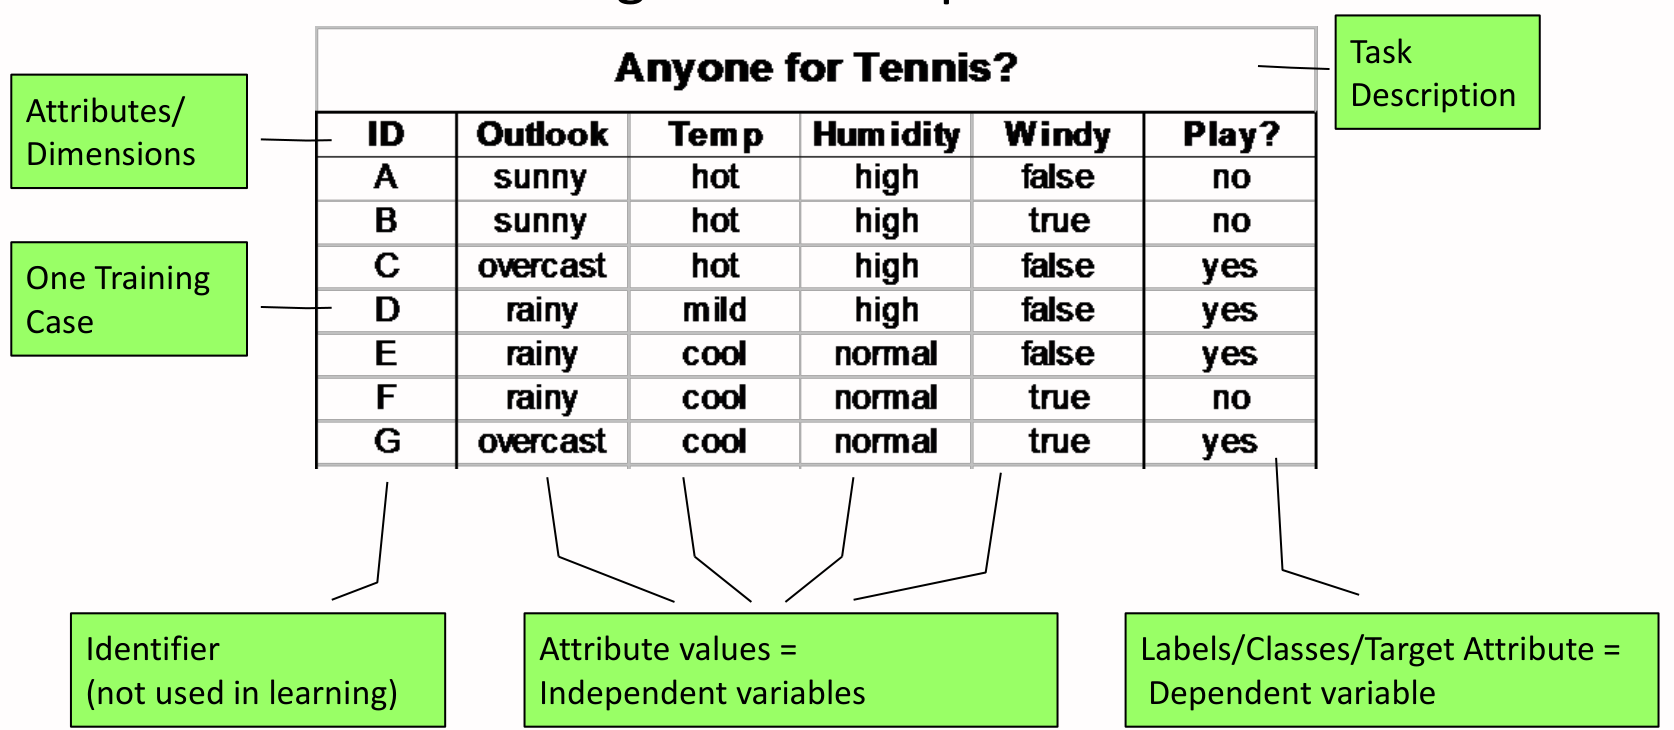
\includegraphics[width=\textwidth]{./images/classification_data_example.png}
    \caption{Training Data Example for a Classification Task}
\end{figure}

\begin{figure}[H]
    \centering
    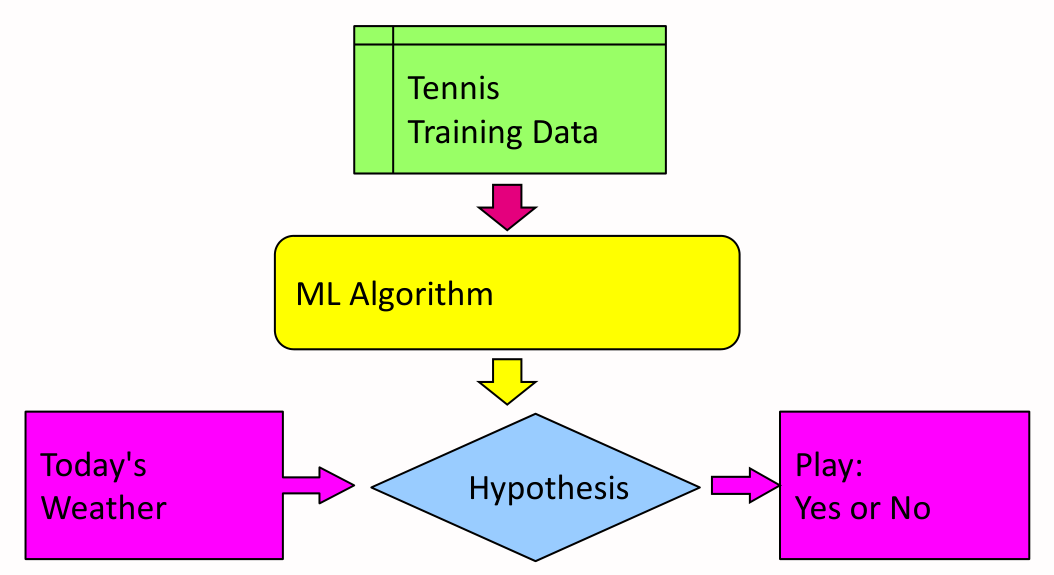
\includegraphics[width=0.6\textwidth]{./images/supervised_learning_overview.png}
    \caption{Overview of the Supervised Learning Process}
\end{figure}

\subsection{Introduction to Classification}
The simplest type of classification task is where instances are assigned to one of two categories: this is referred
to as a \textbf{binary classification task} or two-class classification task.
Many popular machine learning problems fall into this category:
\begin{itemize}
    \item   Is cancer present in a scan? (Yes / No).
    \item   Should this loan be approved? (Yes / No).
    \item   Sentiment analysis in text reviews of products (Positive / Negative).
    \item   Face detection in images (Present / Not Present).
\end{itemize}

The more general form of classification task is the \textbf{mutli-class classification} where the number of classes
is $\geq 3$.

\subsubsection{Example Binary Classification Task}
Objective: build a binary classifier to predict whether a new previously unknown athlete who did not feature in the 
dataset should be drafted.

\begin{minipage}{0.5\textwidth}
    There are 20 examples in the dataset, see \verb|college_athletes.csv| on Canvas.
    \\\\
    The college athlete's dataset contains two attributes: 
    \begin{itemize}
        \item   Speed (continuous variable).
        \item   Agility (continuous variable).
    \end{itemize}

    The target data: whether or not each athlete was drafted to a professional team (yes / no).
\end{minipage}
\hfill
\begin{minipage}{0.5\textwidth}
    \begin{figure}[H]
        \centering
        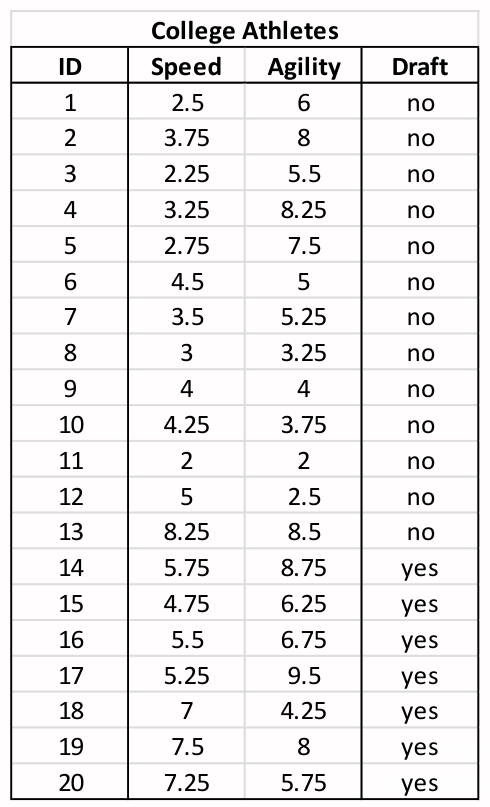
\includegraphics[width=0.6\textwidth]{./images/example_binary_classification.png}
        \caption{Example Dataset for a Binary Classification Task}
    \end{figure}
\end{minipage}

\begin{figure}[H]
    \centering
    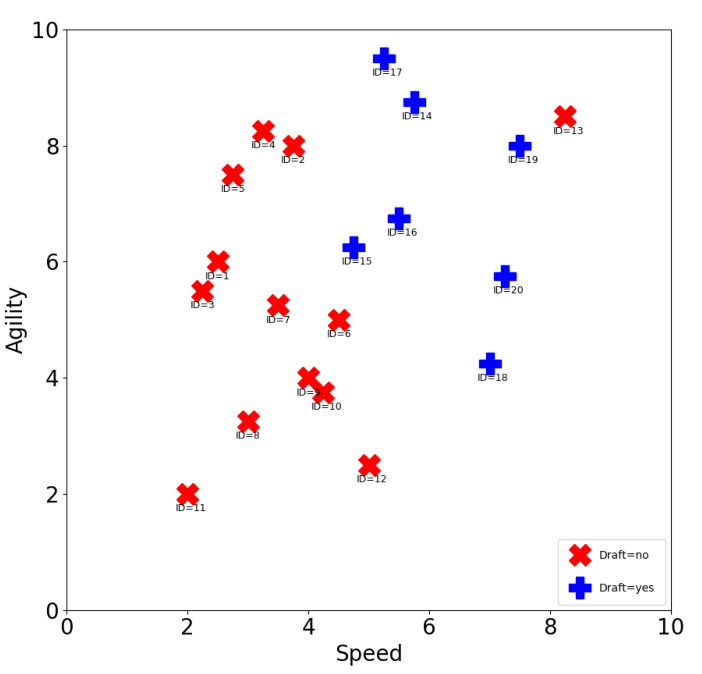
\includegraphics[width=0.6\textwidth]{./images/feature_space_lot_college_athlete.png}
    \caption{Feature Space Plot for the College Athlete's Dataset}
\end{figure}

We want to decide on a reasonable \textbf{decision boundary} to categorise new unseen examples, such as the one
denoted by the purple question mark below.
We need algorithms that will generate a hypothesis / model consistent with the training data.
Is the decision boundary shown below in thin black lines a good one? 
It is consistent with all of the training data, but it was drawn manually; in general, it won't be possible to 
manually draw such decision boundaries when dealing with higher dimensional data (e.g., more than 3 features).

\begin{figure}[H]
    \centering
    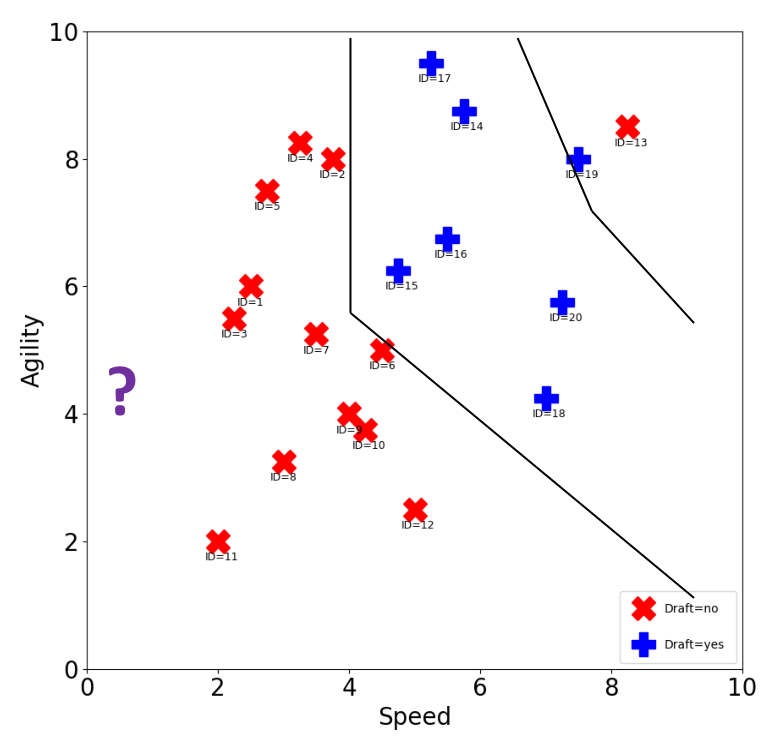
\includegraphics[width=0.5\textwidth]{./images/feature_space_lot_college_athlete_decision_boundary.png}
    \caption{Feature Space Plot for the College Athlete's Dataset}
\end{figure}

\subsubsection{Example Classification Algorithms}
There are many machine learning algorithms available to learn a classification hypothesis / model.
Some examples (with corresponding scikit-learn classes) are:
\begin{itemize}
    \item   $k$-nearest neighbours: scikit-learn \verb|KNeighboursClassifier|.
    \item   Decision trees: scikit-learn \verb|DecisionTreeClassifier|.
    \item   Gaussian Processes: scikit-learn \verb|GaussianProcessClassifier|.
    \item   Neural networks: scikit-learn \verb|MLPClassifier|.
    \item   Logistic regression: scikit-learn \verb|LogisticRegression|.
            Note that despite its name, logistic regression is a linear model for classification rather than regression.
\end{itemize}

\subsubsection{Logistic Regression on the College Athletes Dataset}
Below is an example of a very simple hypothesis generated using an ML model -- a linear classifier created using the
scikit-learn \verb|LogisticRegression| with the default settings.

\begin{figure}[H]
    \centering
    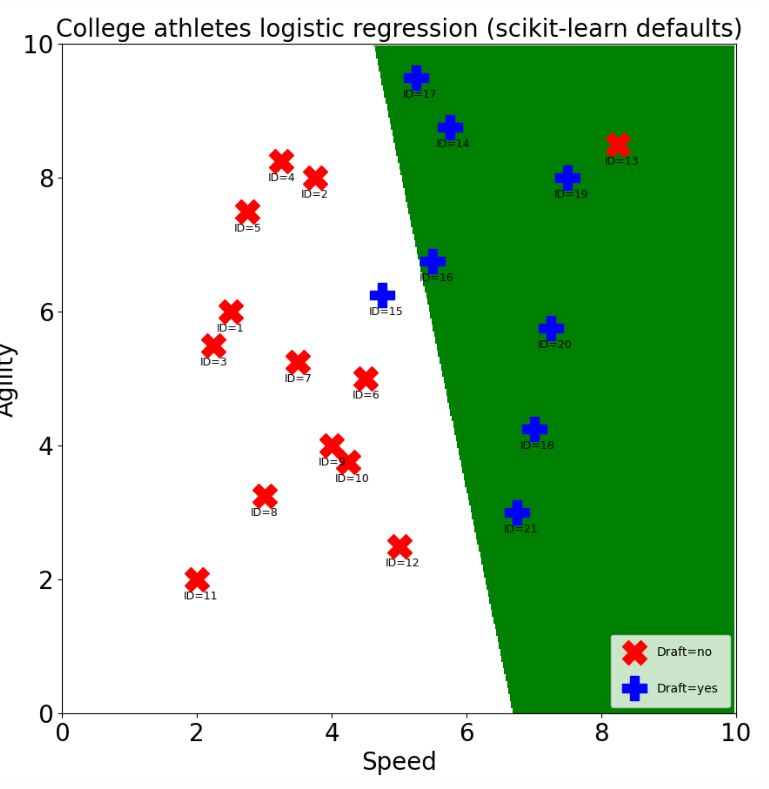
\includegraphics[width=0.5\textwidth]{./images/logistic_regression_college_athletes.png}
    \caption{Logistic Regression on the College Athletes Dataset}
\end{figure}

Is this a good decision boundary?
$\frac{19}{21}$ training examples correct = $90.4\%$ accuracy.
Note how the decision boundary is a straight line (in 2D).
Note also that using logistic regression makes a strong underlying assumption that the data is
\textbf{linearly separable}.

\subsubsection{Decision Tree on the College Athletes Dataset}
Below is an example of a more complex hypothesis, generated using the scikit-learn \verb|DecisionTreeClassifier|
with the default settings.

\begin{figure}[H]
    \centering
    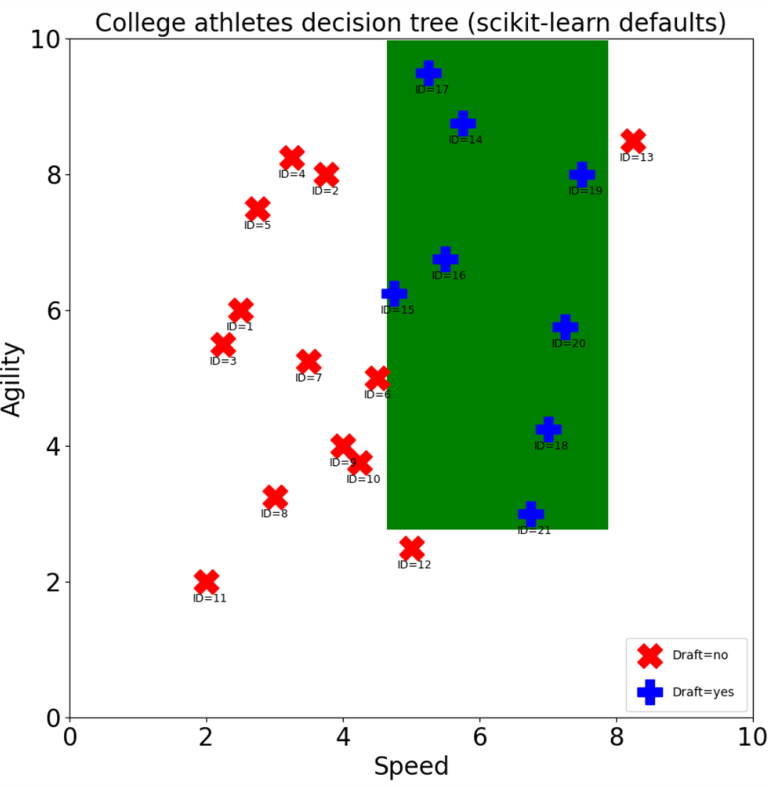
\includegraphics[width=0.5\textwidth]{./images/decision_tree_college_athletes.png}
    \caption{Decision Tree on the College Athletes Dataset}
\end{figure}

Note the two linear decision boundaries: this is a very different form of hypothesis compared to logistic
regression.
Is this a good decision boundary?
$\frac{21}{21}$ training examples correct = $100\%$ accuracy.

\subsubsection{Gaussian Process on the College Athletes Dataset}
Below is an example of a much more complex hypothesis generated using the scikit-learn 
\verb|GaussianProcessClassifier| with the default settings.

\begin{figure}[H]
    \centering
    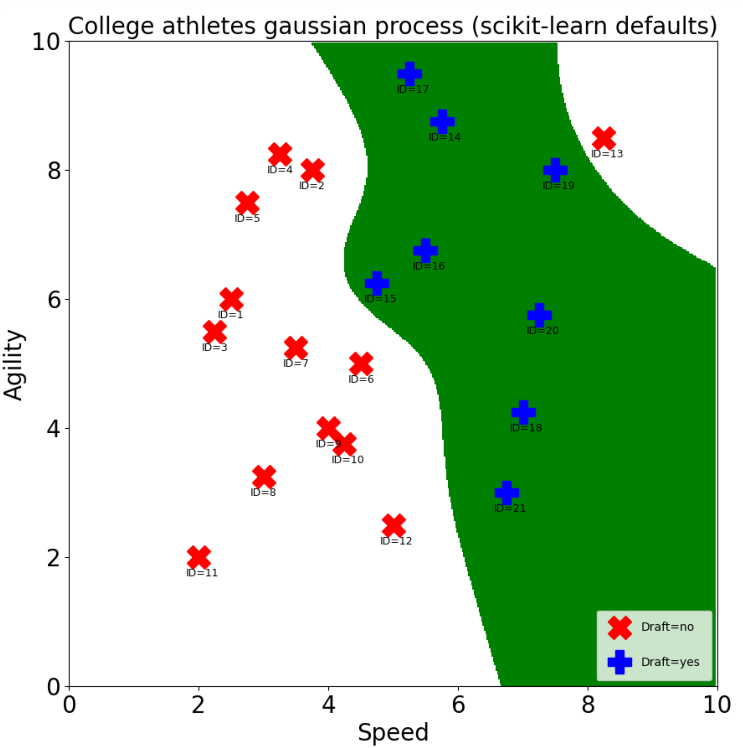
\includegraphics[width=0.5\textwidth]{./images/gaussian_process_college_athletes.png}
    \caption{Gaussian Process on the College Athletes Dataset}
\end{figure}

Note the smoothness of the decision boundary compared to the other methods.
Is this a good decision boundary?
$\frac{21}{21}$ training examples correct = $100\%$ accuracy.
\\\\
Which of the three models explored should we choose?
It's complicated; we need to consider factors such as accuracy of the training data \& independent test data,
complexity of the hypothesis, per-class accuracy etc.

\subsubsection{Use of Independent Test Data}
Use of separate training \& test datasets is very important when developing an ML model.
If you use all of your data for training, your model could potentially have good performance on the training data
but poor performance on new independent test data.


\section{$k$-Nearest Neighbours Algorithm}
\textbf{$k$-nearest neigbours} (or $k$-NN) is one of the simplest machine learning algorithms.
It generates a hypothesis using a very simple principle: predictions for the label or value assigned to a \textit{query instance} should be made based on the most \textit{similar} instances in the training dataset.
Hence, this is also known as \textbf{similarity-based learning}.
\\\\
$k$-NN can be used for both classificatoin \& regression tasks, although for now we will focus only on its application to classification tasks using the scikit-learn implementation \mintinline{python}{KNeighborsClassifier}.

\begin{figure}[H]
    \centering
    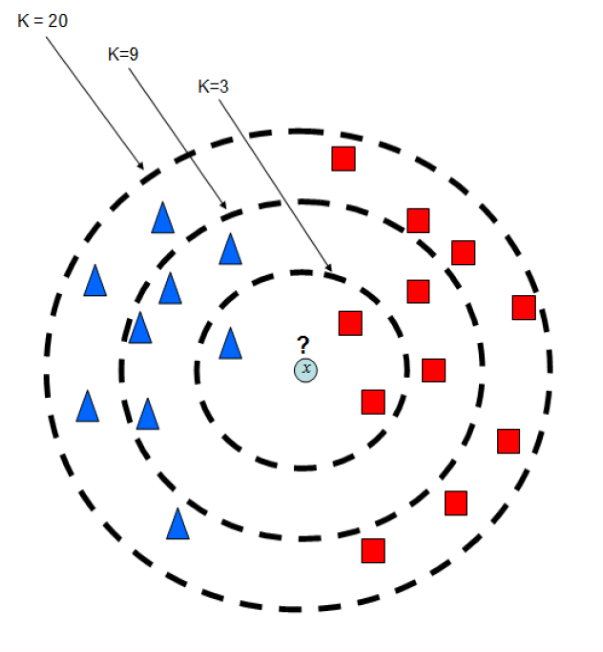
\includegraphics[width=0.5\textwidth]{images/knn.png}
    \caption{$K$-Nearest Neighbour Example}
\end{figure}

The operation of the $k$-NN algorithm is relatively easy to appreciate.
The key insight is that each example is a point in the feature space.
If samples are close to each other in the feature space, they should be close in their target values.
This is related to \textit{code-based reasoning}.
When you want to classify a new \textbf{query case}, you compare it to the stored set and retrieve the $k$ most similar instances.
The query case is the given a label based on the most similar instances.
\\\\
The prediction for a query case is based on several ($k$) nearest neighbours.
We compute the similarity of the query case to all stored cases, and pick the nearest $k$ neighbours;
the simplest way to do this is to sort the instances by distance and pick the lowest $k$ instances.
A more efficient way of doing this would be to identify the $k$ nearest instances in a single pass through the list of distances.
The $k$ nearest neighbours then vote on the classification of the test case: prediction is the \textbf{majority} class voted for.

\subsection{The Nearest Neighbour Algorithm}
The \textbf{1-nearest neighbour algorithm} is the simplest similarity-based / instance-based method.
There is no real training phase, we just store the training cases.
Given a query case with a value to be predicted, we compute the distance of the query case from all stored instances and select the nearest neighbour case.
We then assign the test case the same label (class or regression value) as its nearest neighbour.
The main problem with this approach is susceptibility to noise; to reduce susceptibility to noise, use more than one neighbour, i.e., the $k$-nearest neighbours algorithm.
\\\\
1NN with Euclidean distance as the distance metric is equivalent to partitioning the feature space into a \textbf{Voronoi Tessellation}:
finding the predicted target class is equivalent to finding which Voronoi region it occupies.

\begin{figure}[H]
    \centering
    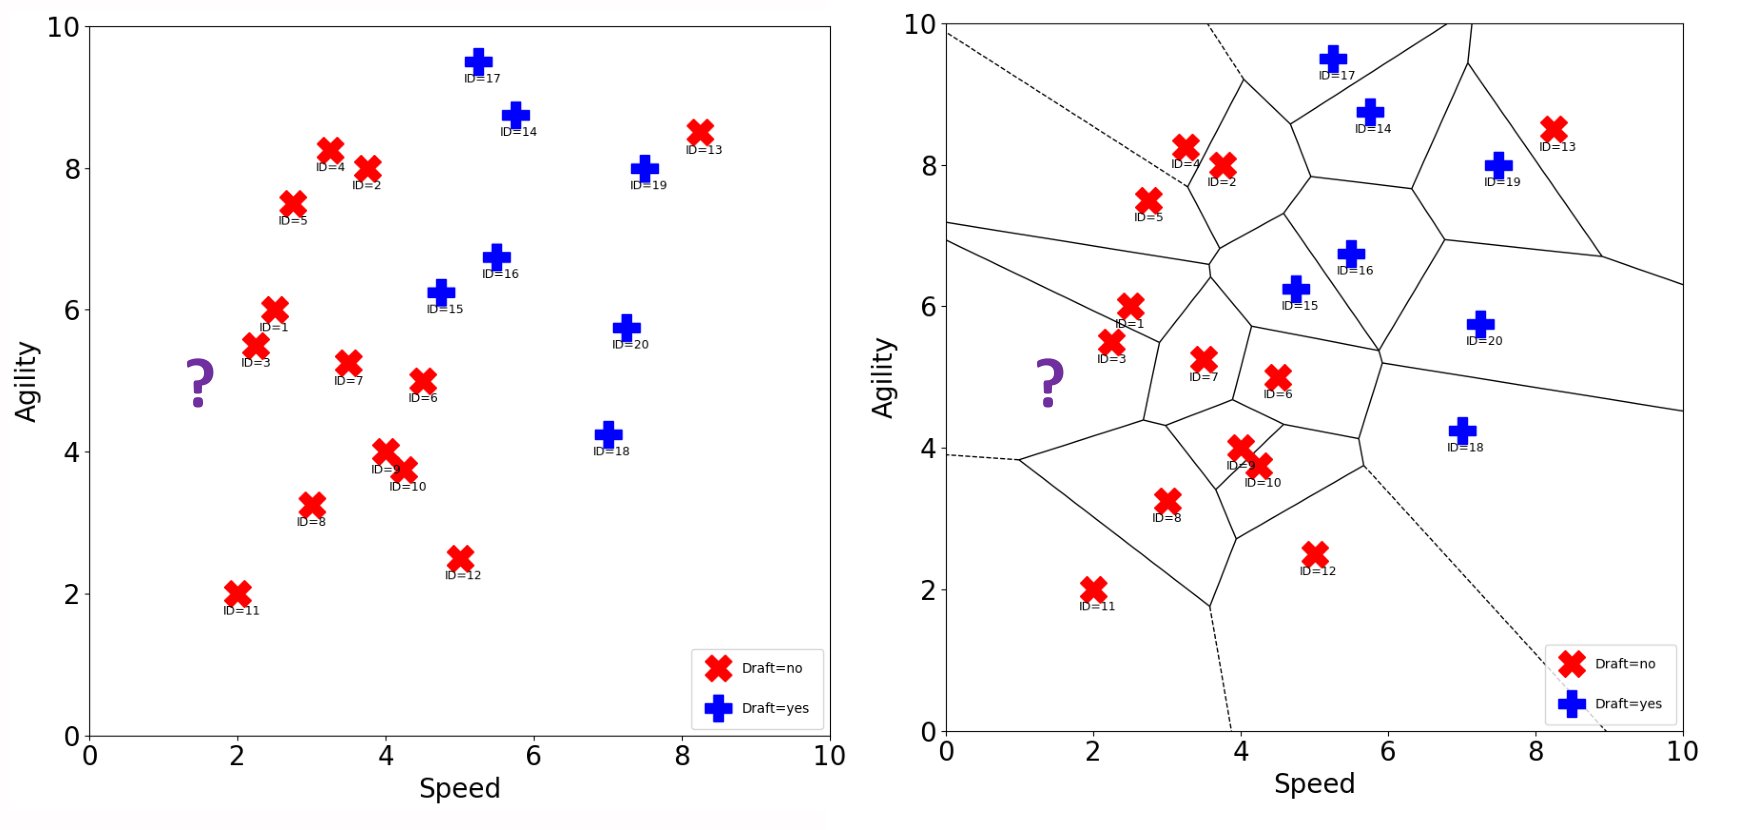
\includegraphics[width=0.9\textwidth]{images/voronoi.png}
    \caption{Feature Space Plot (left) \& Corresponding Voronoi Tesselation (right)}
\end{figure}

\begin{figure}[H]
    \centering
    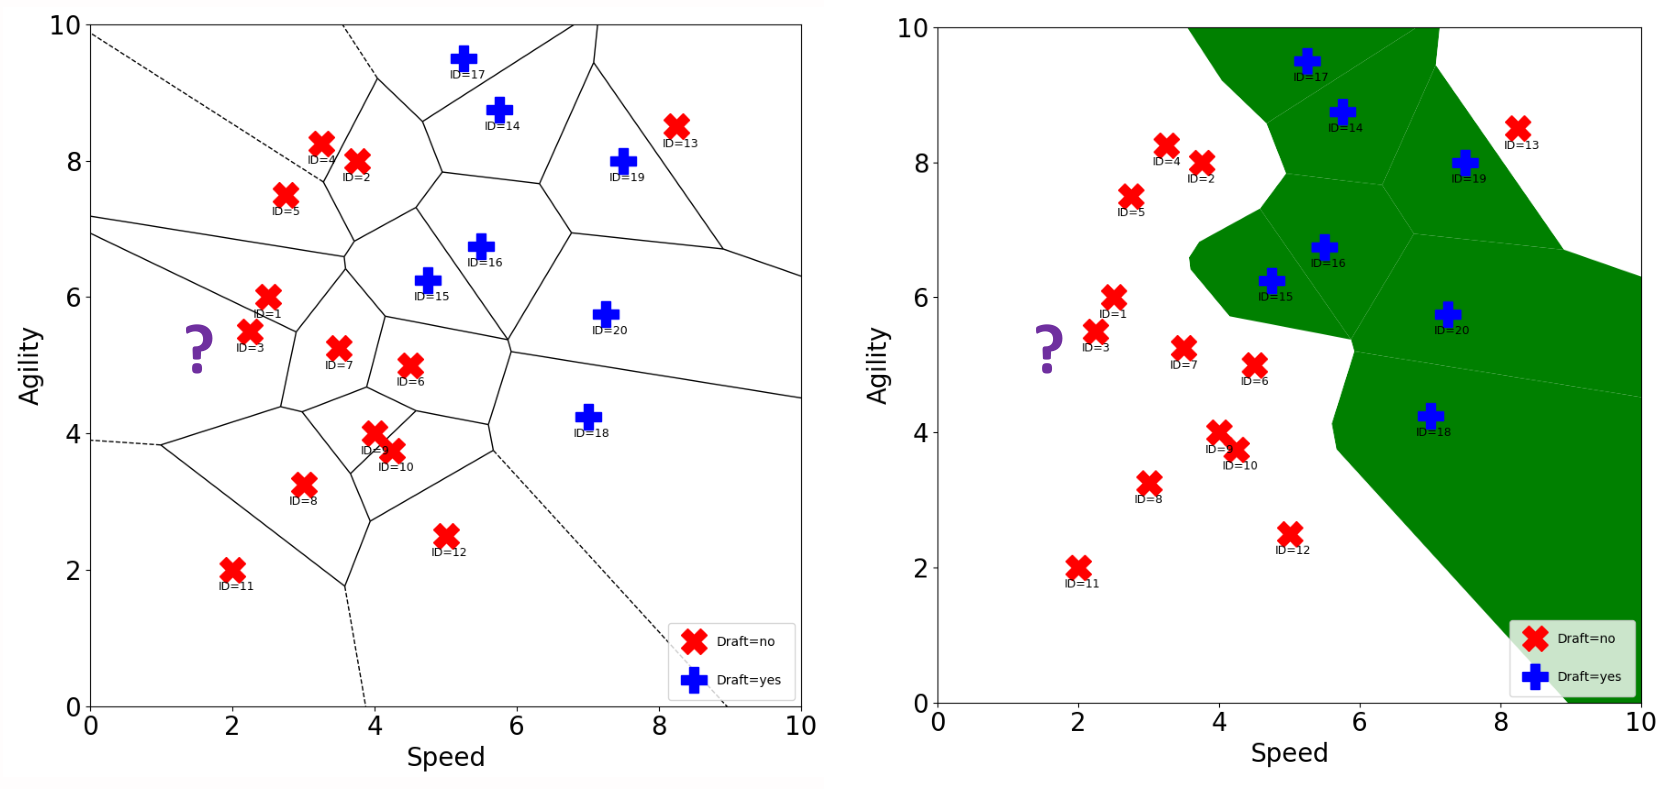
\includegraphics[width=0.9\textwidth]{images/1nnboundary.png}
    \caption{1NN Decision Boundary from Voronoi Tessellation}
\end{figure}

\begin{figure}[H]
    \centering
    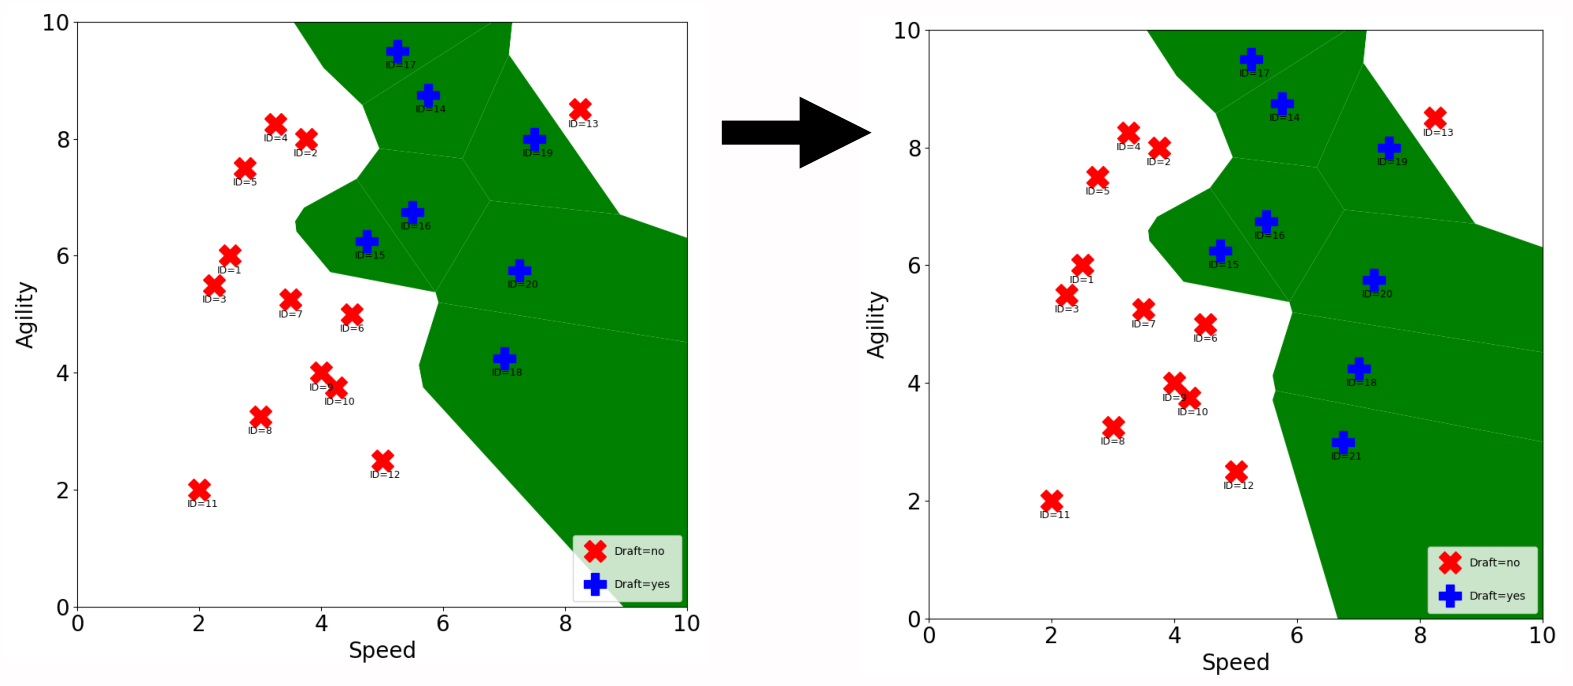
\includegraphics[width=0.9\textwidth]{images/morevoronoi.png}
    \caption{Effect of Adding More Training Data to Voronoi Tessellation}
\end{figure}

\subsection{$k$-NN Hyperparameters}
The $k$-NN algorithm also introduces a new concept to us that is very important for ML algorithms in general: hyperparameters.
In ML algorithms, a \textbf{hyperparameter} is a parameter set by the user that is used to control the behaviour of the learning process.
Many ML algorithms also have other parameters that are set by the algorithm during its learning process (e.g., the weights
assigned to connections between neurons in an artificial neural network).
Examples of hyperparameters include:
\begin{itemize}
    \item   Learning rate (typically denoted using the Greek letter $\alpha$).
    \item   Topology of a neural network (the number \& layout of neurons).
    \item   The choice of optimiser when updating the weights of a neural network.
\end{itemize}

Many ML algorithms are very sensitive to the choice of hyperparameters: poor choice of values yields poor performance.
Therefore, hyperparameter tuning (i.e., determining the values that yield the best performance) is an important topic in ML.
However, some simple ML algorithms do not have any hyperparameters.
\\\\
$k$-NN has several key hyperparameters that we must choose before applying it to a dataset:
\begin{itemize}
    \item   The number of neighbours $k$ to take into account when making a prediction: \mintinline{python}{n_neighbours} in the scikit-learn implementation of \mintinline{python}{KNeighboursClassifier}.
    \item   The method used to measure how similar instances are to one another: \mintinline{python}{metric} in scikit-learn.
\end{itemize}

\subsection{Measuring Similarity}
\subsubsection{Measuring Similarity Using Distance}
Consider the college athletes dataset from earlier.
How should we measure the similarity between instances in this case?
\textbf{Distance} is one option: plot the points in 2D space and draw a straight line between them.
We can think of each feature of interest as a dimension in hyperspace.
\\\\
A \textbf{metric} or distance function may be used to define the distance between any pair of elements in a set.
$\text{metric}(a,b)$ is a function that returns the distance between two instances $a$ \& $b$ in a set.
$a$ \& $b$ are vectors containing the values of the attributes we are interested in for the data points we wish to measure between.

\subsubsection{Euclidean Distance}
\textbf{Euclidean distance} is one of the best-known distance metrics.
It computes the length of a straight line between two points.
$$
\text{Euclidean}(a,b) = \sqrt{\sum^m_{i=1}(a[i] - b[i])^2}
$$

Here $m$ is the number of features / attributes to be used to calculate the distance (i.e., the dimensions of the vectors $a$ \& $b$).
Euclidean distance calculates the square root of the sum of squared differences for each feature.

\subsubsection{Manhattan Distance}
\textbf{Manhattan distance} (also known as ``taxicab distance'') is the distance between two points measured along axes at
right angles.
$$
\text{Manhattan}(a,b) = \sum^m_{i=1}\text{abs}(a[i] - b[i])
$$

As before, $m$ is the number of features / attributes to be used to calculate the distance (i.e., the dimension of the vectors $a$ \& $b$) and $\text{abs}()$ is a function which returns the absolute value of a number.
Manhattan distance calculates the sum of the absolute differences for each feature.

\begin{tcolorbox}[colback=gray!10, colframe=black, title=\textbf{Example: Calculating Distance}]
    Calculate the distance between $d_{12} = [5.00, 2.50]$ \& $d_5 = [2.75, 7.50]$.
    $$
    \text{Euclidean}(d_{12}, d_5) = \sqrt{(5.00 - 2.75)^2 + (2.50 - 7.50)^2} = 5.483
    $$
    $$
    \text{Manhattan}(d_{12}, d_5) = \text{abs}(5.00 - 2.75) + \text{abs}(2.50 - 7.50) = 7.25
    $$

    \begin{figure}[H]
        \centering
        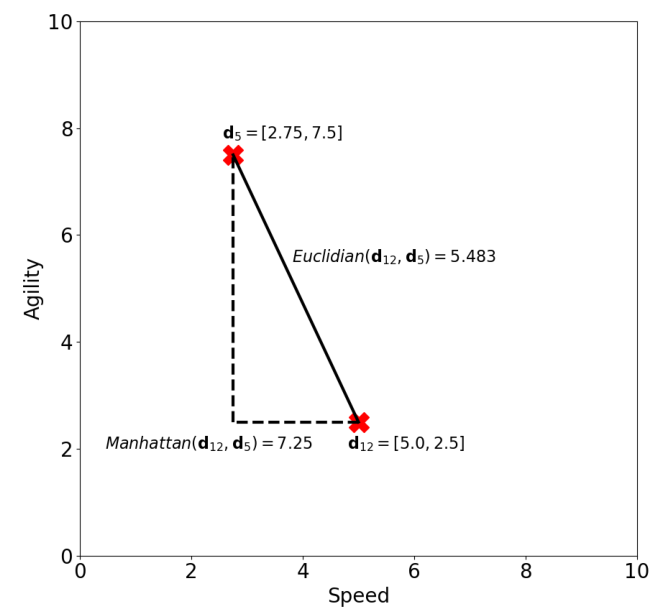
\includegraphics[width=0.5\textwidth]{./images/calc_distance_example.png}
        \caption{Euclidean vs Manhattan Distance}
    \end{figure}
\end{tcolorbox}

\subsubsection{Minkowski Distance}
The \textbf{Minkowski distance} metric generalises both the Manhattan distance and the Euclidean distance metrics.
$$
\text{Minkowski}(a,b) = \left( \sum^m_{i=1} \text{abs}(a[i] - b[i])^p \right)^{\frac{1}{p}}
$$
As before, $m$ is the number of features / attributes to be used to calculate the distance (i.e., the dimension of the vectors $a$ \& $b$).
Minkowski distance calculates the absolute value of the differences for each feature.

\subsubsection{Similarity for Discrete Attributes}
Thus far we have considered similarity measures that only apply to continuous attributes\footnote{Note that discrete/continuous attributes are not to be confused with classification/regression}.
Many datasets have attributes that have a finite number of discrete values (e.g., Yes/No or True/False, survey responses, ratings).
One approach to handling discrete attributes is \textbf{Hamming distance}: the Hamming distance is calculated as 0 for each attribute where both cases have the same value and 1 for each attribute where they are different.
E.g., Hamming distance between the strings ``Ste\colorbox{yellow}{phe}n'' and ``Ste\colorbox{yellow}{fan}n'' is 3.

\subsubsection{Comparison of Distance Metrics}
Euclidean \& Manhattan distance are the most commonly used distance metrics although it is possible to define infinitely many distance metrics using the Minkowski distance.
Manhattan distance is cheaper to compute than Euclidean distance as it is not necessary to compute the squares of differences and a square root, so Manhattan distance may be a better choice for very large datasets if computational resources are limited.
It's worthwhile to try out several different distance metrics to see which is the most suitable for the dataset at hand.
Many other methods to measure similarity also exist, including cosine similarity, Russel-Rao, Sokal-Michener.

\subsection{Choosing a Value for $k$}
The appropriate value for $k$ is application dependent, and experimentation is needed to find the optimal value.
Typically, it is $> 3$ and often in the range $5$ -- $21$.
Increasing $K$ has a \textbf{smoothing effect}:
\begin{itemize}
    \item   If $k$ is too low, it tends to overfit if the data is noisy.
    \item   If $k$ is too high, it tends to underfit.
\end{itemize}

In imbalanced datasets, the majority target class tends to dominate for large $k$ values.
It's important to note that $k$ does not affect computational cost much: most of the computation is in calculating the distances from the query to all stored instances.

\begin{figure}[H]
    \centering
    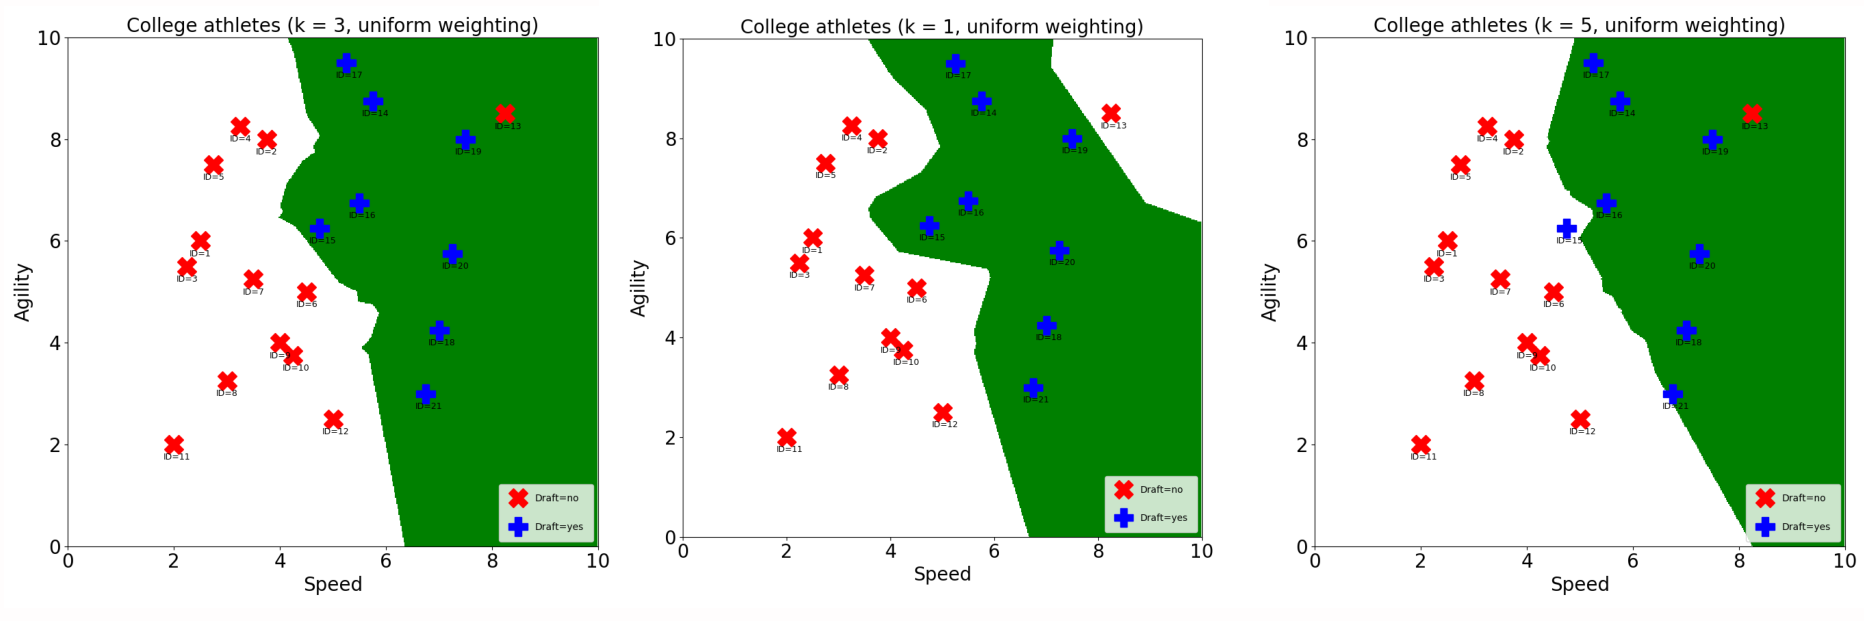
\includegraphics[width=\textwidth]{images/increasingk.png}
    \caption{Effect of Increasing $k$ (1)}
\end{figure}

\begin{figure}[H]
    \centering
    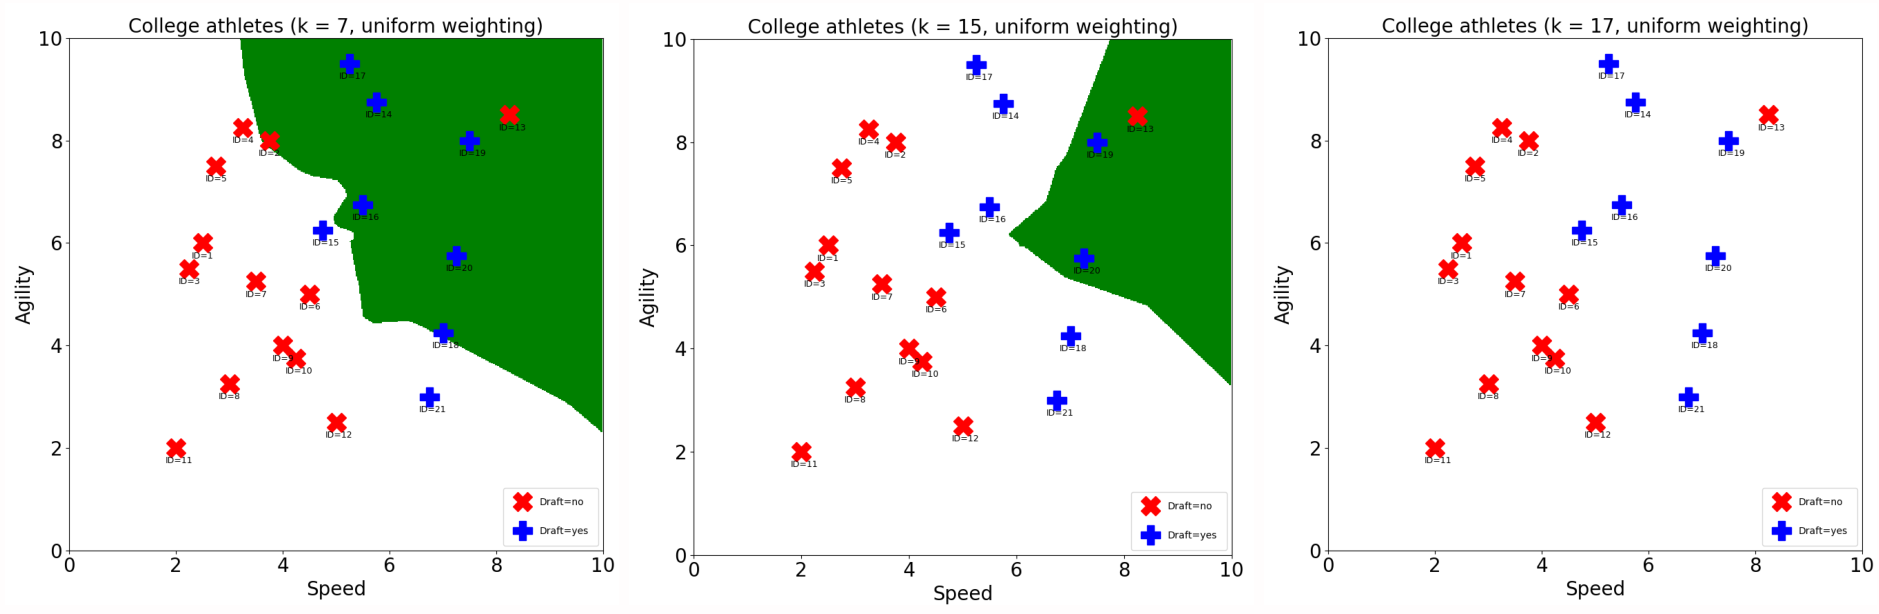
\includegraphics[width=\textwidth]{images/increasingk2.png}
    \caption{Effect of Increasing $k$ (2)}
\end{figure}

\begin{figure}[H]
    \centering
    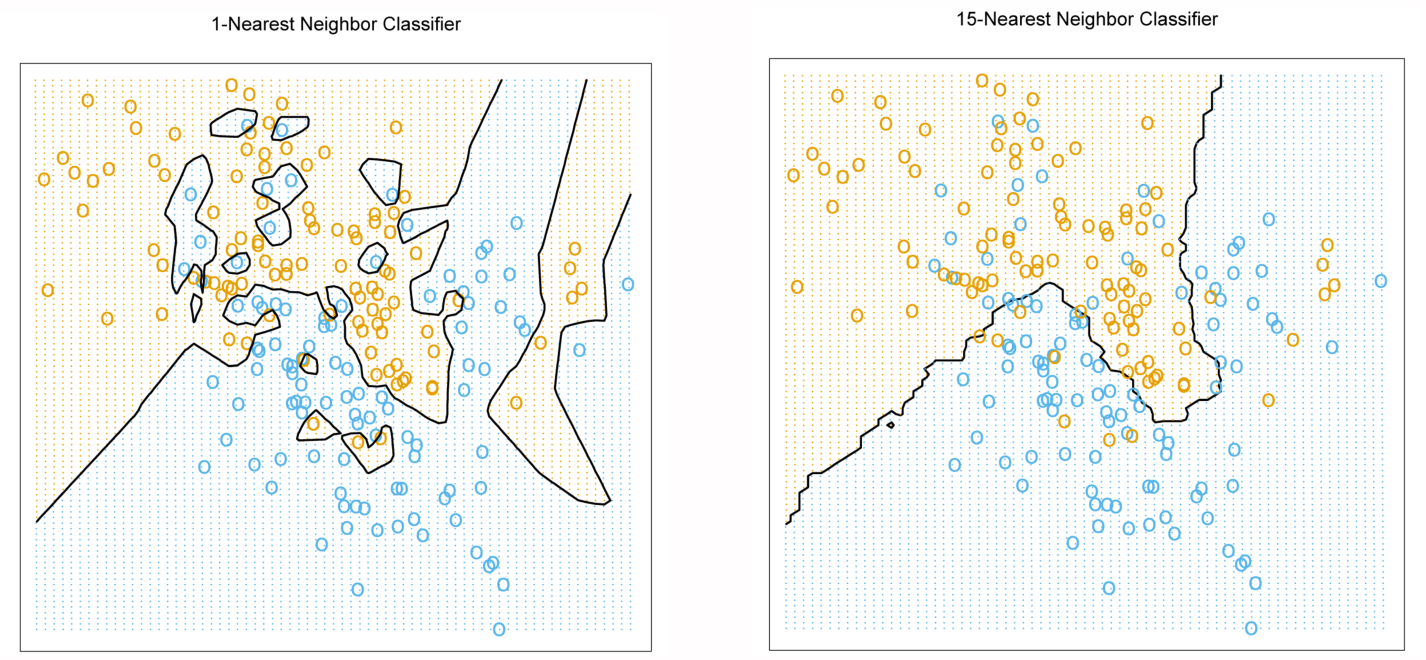
\includegraphics[width=\textwidth]{images/smoothingeffectk.png}
    \caption{Smoothing Effect of $k$}
\end{figure}

\subsubsection{Distance-Weighted $k$-NN}
In \textbf{distance-weighted $k$-NN}, we give each neighbour a weight equal to the inverse of its distance from the target.
We then take the weighted vote or weighted average to classify the target case.
It's reasonable to use $k = [\text{all training cases}]$.

\begin{figure}[H]
    \centering
    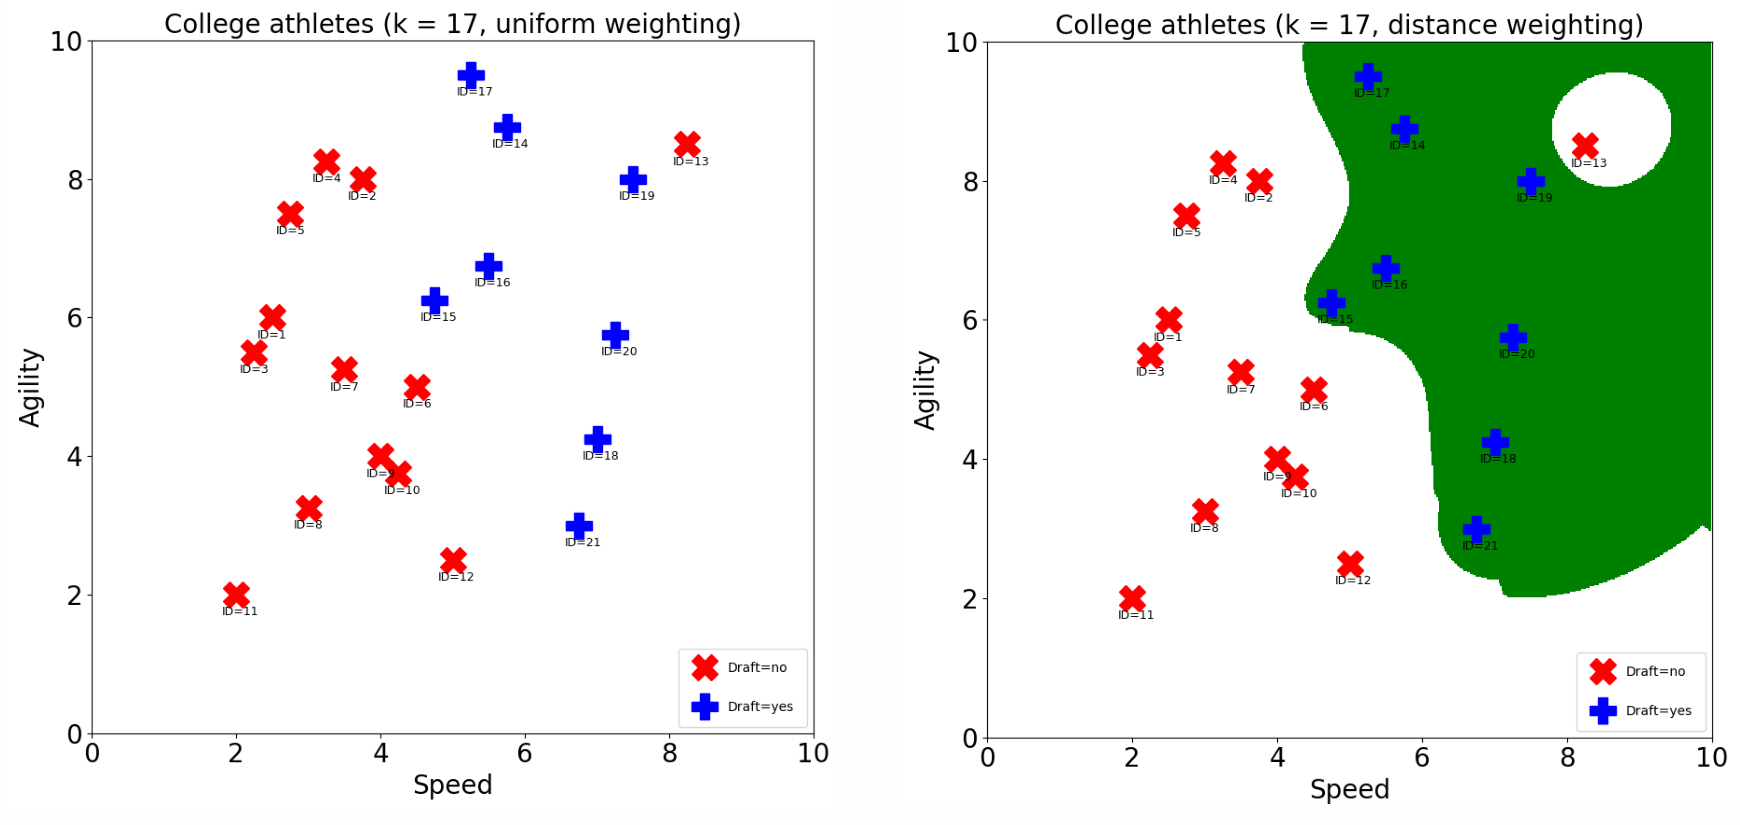
\includegraphics[width=\textwidth]{images/distanceweightingknn.png}
    \caption{Effect of Distance Weighting}
\end{figure}

\section{Decision Trees}
\textbf{Decision trees} are a fundamental structure used in information-based machine learning.
The idea is to use a decision tree as a predictive model to decide what category/label/class an item belongs to based on the values of its features.
Decision trees consist of \textbf{nodes} (where two branches intersect) which are decision points which partition the data.
Observations about an item (values of features) are represented using branches.
The terminal nodes are called \textbf{leaves} and specify the target label for an item.
The inductive learning of a decision tree is as follows:
\begin{enumerate}
    \item   For all attributes that have not yet been used in the tree, calculate their impurity (\textbf{entropy} or \textbf{Gini index}) and \textbf{information/Gini gain} values for the training samples.
    \item   Select the attribute that has the \textbf{highest} information gain.
    \item   Make a tree node containing that attribute.
    \item   This node \textbf{partitions} the data: apply the algorithm recursively to each partition.
\end{enumerate}

The main class used in scikit-learn to implement decision tree learning for classification tasks is \mintinline{python}{DecisionTreeClassifier}.
The default measure of impurity is the Gini index, but entropy is also an option.

\subsection{Computing Entropy}
We already saw how some descriptive features can more effectively discriminate between (or predict) classes which are present in the dataset.
Decision trees partition the data at each node, so it makes sense to use features which have higher discriminatory power ``higher up'' in a decision tree.
Therefore, we need to develop a formal measure of the discriminatory power of a given attribute.
\\\\
Claude Shannon (often referred to as ``the father of information theory'') proposed a measure of the impurity of the elements in the set called \textbf{entropy}.
Entropy may be used to measure the uncertainty of a random variable.
The term ``entropy'' generally refers to disorder or uncertainty, so the use of this term in the context of information theory is analogous to other well-known uses of the term such as in statistical themodynamics.
The acquisition of information (\textbf{information gain}) corresponds to a \textbf{reduction in entropy}.
\\\\
The \textbf{entropy} of a dataset $S$ with $n$ different classes may be calculated as:
\[
    \text{Ent}(S) = \sum^n_{i=1} -p_i \log_2 p_i
\]
where $p_i$ is the proportion of the class $i$ in the dataset.
This is an example of a probability mass function.
Entropy is typically measured in \textbf{bits} (note the $\log_2$ in the equation above):
the lowest possible entropy output from this function is 0 ($\log_2 1 = 0$), while the highest possible entropy is $\log_2n$ (which is equal to 1 when there are only two classes).
\\\\
We use the binary logarithm because a useful measure of uncertainty should assign high uncertainty to outcomes with a low probability and assign low uncertainty values to outcomes with a high probability.
$\log_2$ returns large negative values when $P$ is close to 0 and small negative values when $P$ is close to 1.
We use $-\log_2$ for convenience, as it returns positive entropy values with 0 as the lowest entropy.

\begin{tcolorbox}[colback=gray!10, colframe=black, title=\textbf{Worked Entropy Example}]
    \begin{figure}[H]
        \centering
        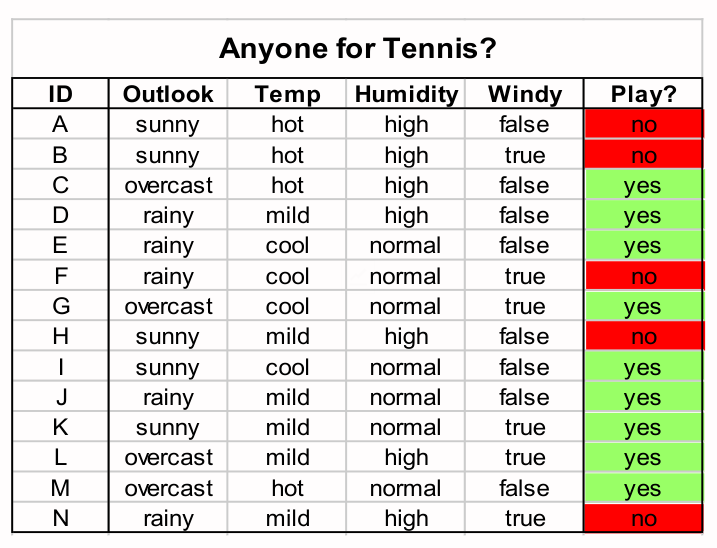
\includegraphics[width=0.6\textwidth]{images/anyonefortennis.png}
        \caption{Example Data}
    \end{figure}

    Workings;
    \begin{align*}
        \text{Ent}(S)   =& \text{Ent}([9+, 5-]) \\
                        =& \frac{-9}{14} \log_2 \left( \frac{9}{14} \right) - \frac{5}{14} \log_2 \left( \frac{5}{14} \right) \\
                        =& 0.9403
    \end{align*}

    Note that if you are calculating entropy using a spreadsheet application such as Excel, make sure that you are using $\log_2$, e.g. \verb|LOG(9/14,2)|.
\end{tcolorbox}

\subsection{Computing Information Gain}
The \textbf{information gain} of an attribute is the reduction of entropy from partitioning the data according to that attribute:
\[
    \text{Gain}(S,A) = \text{Ent}(S) - \sum_{v \in \text{Values}(A)} \frac{\left| S_v \right|}{\left| S \right|} \text{Ent}(S_v)
\]

Here $S$ is the entire set of data being considered and $S_v$ refers to each partition of the data according to each possible value $v$ for the attribute.
$\left| S \right|$ \& $\left| S_v \right|$ refer to the cardinality or size of the overall dataset, and the cardinality or size of a partition respectively.
When selecting an attribute for a node in a decision tree, we use whichever attribute $A$ that gives the greatest information gain.

\begin{tcolorbox}[colback=gray!10, colframe=black, title=\textbf{Worked Information Gain Example}]
    Given $\left| S \right| = 14$, $\left| S_{\text{windy} = \text{true}} \right| = 6$, \& $\left| S_{\text{windy} = \text{false}} \right| = 8$, calculate the information gain of the attribute ``windy''.

    \begin{align*}
        \text{Gain}(S, \text{windy}) =& \text{Ent}(S) - \frac{\left| S_{\text{windy} = \text{true}} \right|}{\left| S \right|} \text{Ent}(S_\text{windy} = \text{true})
        -  \frac{\left| S_{\text{windy} = \text{false}} \right|}{\left| S \right|} \text{Ent}(S_\text{windy} = \text{false}) \\
        =& \text{Ent}(S) - \left( \frac{6}{14} \right) \text{Ent}(\left[3+,3-\right]) - \left( \frac{8}{14} \right) \text{Ent}(\left[ 6+,2- \right]) \\
        =& 0.940 - \left( \frac{6}{14} \right) 1.00 - \left( \frac{8}{14} \right) 0.811\\
        =& 0.048
    \end{align*}
\end{tcolorbox}

The best partitioning is the one that results in the highest information gain.
Once the best split for the root node is found, the procedure is repeated with each subset of examples.
$S$ will then refer to the subset in the partition being considered instead of the entire dataset.

\subsection{Computing the Gini Index}
An alternative to using entropy as the measure of the impurity of a set is to use the \textbf{Gini Index}:
\[
    \text{Gini}(S) = 1 - \sum^n_{i=1} p_i^2
\]

This is the default measure of impurity in scikit-learn.
The gain for a feature can then be calculated based off the reduction in the Gini Index (rather than as a reduction in entropy):
\[
    \text{GiniGain}(S,A) = \text{Gini}(S) = \sum_{v \in \text{Values}(A)} \frac{\left| S_v \right|}{\left|S\right|}\text{Gini}(S_v)
\]

\subsection{The ID3 Algorithm}
\begin{algorithm}[H]
\caption{ID3 Algorithm}
\begin{algorithmic}[1]
\Procedure{ID3}{Examples, Attributes, Target}
    \State \textbf{Input:} 
    \State \quad Examples: set of classified examples
    \State \quad Attributes: set of attributes in the examples
    \State \quad Target: classification to be predicted
    \If{Examples is empty}
        \State \Return Default class
    \ElsIf{all Examples have the same class}
        \State \Return this class
    \ElsIf{all Attributes are tested}
        \State \Return majority class
    \Else
        \State Let Best = attribute that best separates Examples relative to Target
        \State Let Tree = new decision tree with Best as root node
        \ForAll{value $v_i$ of Best}
            \State Let Examples$_i$ = subset of Examples where Best = $v_i$
            \State Let Subtree = ID3(Examples$_i$, Attributes - Best, Target)
            \State Add branch from Tree to Subtree with label $v_i$
        \EndFor
        \State \Return Tree
    \EndIf
\EndProcedure
\end{algorithmic}
\end{algorithm}

\subsection{Decision Tree Summary}
Decision trees are popular because:
\begin{itemize}
    \item   It's a relatively easy algorithm to implement.
    \item   It's fast: greedy search without backtracking.
    \item   It has comprehensible output, which is important in decision-making (medical, financial, etc.).
    \item   It's practical.
    \item   It's \textbf{expressive:} a decision tree can technically represent any boolean function, although some functions require exponentially large trees such as a parity function.
\end{itemize}

\subsubsection{Dealing with Noisy or Missing Data}
If the data is inconsistent or \textit{noisy} we can either use the majority class as in line 11 of the above ID3 algorithm, or interpret the values as probabilities, or return the average target feature value.







\end{document}
